\begin{frame}
  \frametitle{Gastos del GNC}
  \vspace{-0.25cm}
  {\centering\small\color{blue!70!black}Fuente: MHCP y CARF\par}
  \vspace{-0.1cm}
  \begin{center}
    \resizebox{0.88\textwidth}{!}{
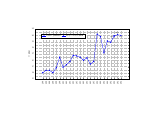
\begin{tikzpicture}[scale=0.08]
\begin{axis}[
    width=16.5cm,
    height=9.5cm,
    ylabel={\% PIB},
    xtick={1,...,24},
    xticklabels={2004,2005,2006,2007,2008,2009,2010,2011,2012,2013,2014,2015,2016,2017,2018,2019,2020,2021,2022,2023,2024,2025,2026,2027},
    x tick label style={rotate=90, anchor=east},
    ymin=13,
    ymax=21,
    grid=both,
    grid style=dashed,
    minor y tick num=1,
    legend style={at={(0.3,0.9)}, anchor=north, legend columns=-1},
    thick
]

% Gasto Primario
\addplot[
    color=blue,
    mark=*,
    very thick
] coordinates {
    (1,14.0) (2,14.4) (3,14.4) (4,14.0) (5,14.8) (6,16.5) (7,14.9) (8,15.3)
    (9,15.8) (10,16.8) (11,16.7) (12,16.5) (13,16.0) (14,16.4) (15,15.4) (16,15.8)
    (17,20.2) (18,19.8) (19,17.2) (20,19.1) (21,18.9) (22,19.9)
};

% Proyección CARF 2026--2027
\addplot[
    color=blue,
    mark=*,
    very thick,
    densely dotted
] coordinates {
    (22,19.9) (23,20.1) (24,20.0)
};

%% Gasto Total
%\addplot[
%    color=red,
%    mark=square*,
%    dashed
%] coordinates {
%    (1,17.6) (2,17.5) (3,18.1) (4,17.8) (5,18.0) (6,19.5) (7,17.6) (8,18.0)    (9,18.4) (10,19.1) (11,18.9) (12,19.1) (13,18.9) (14,19.3) (15,18.2) (16,18.7) (17,23.1) (18,23.1) (19,21.5) (20,22.9) (21,23.2) (22,22.7)
%};

% Señalar GP 2019 y GP 2025
\node[anchor=south west] at (axis cs:16,15.8) {\scriptsize  15.8};
\node[anchor=north east] at (axis cs:22,19.9) {\scriptsize  19.9};
\node[anchor=south] at (axis cs:23,20.1) {\scriptsize  20.1};
\node[anchor=north] at (axis cs:24,20.0) {\scriptsize  20.0};

\legend{Gasto primario, Proyección CARF}
\end{axis}
\end{tikzpicture}
}
  \end{center}
  \note{[Sources] MHCP, serie histórica utilizada en la presentación, 2004--2025. CARF, Informe de análisis técnico al MFMP 2026, cuadros 1 y 5, junio de 2026. Proyecciones de gasto primario: 20,1\% del PIB en 2026 y 20,0\% en 2027.}
\end{frame}
